%! TEX root = ../../master.tex
\lecture[Überlagerungen von CW-Komplexen. Untergruppen von freien Gruppen. Konstruktion von CW-Komplexen mit beliebiger Fundamentalgruppe. Borsuk-Ulam. Ausblick auf Topologie I und II: $\pi_n$, Homologie, Kohomologie.]{Sa 18 Sep 2021}{Fundamentalgruppen von CW-Komplexen}

\begin{theorem}\label{thm:überlagerung-von-cw-komplex-ist-überlagerung}
    Jede Überlagerung eines CW-Komplexes ist ein CW-Komplex. Insbesondere ist eine Überlagerung eines Graphen wieder ein Graph.
\end{theorem}
%\begin{rproof}{thm:überlagerung-von-cw-komplex-ist-überlagerung}[skizziert]
%    Sei $X$ ein CW-Komplex und  $p\colon E \to  X$ eine Überlagerung.
%\[
%    \begin{tikzcd}
%        & E \ar{d}{p} \\
%        \underbrace{c_{α}}_{\text{zusammenziehbar}} \ar[dashed]{ur}\ar{r} & X 
%    \end{tikzcd}
%\]
%Da die $k$-Zellen von  $X$ zusammenziehbar sind, existiert jeweils eine Hebung  $\tilde{φ}_α\colon c_α \to  E$. Die Hebung solch einer $k$-Zelle von $X$ ist eine $k$-Zelle, also ergibt sich eine CW-Komplex Struktur auf $E$.
%\end{rproof}

\begin{example}
    Betrachte die Überlagerung $S^1 \to  S^1$ gegeben durch $z \mapsto z^2$, d.h.
\[
    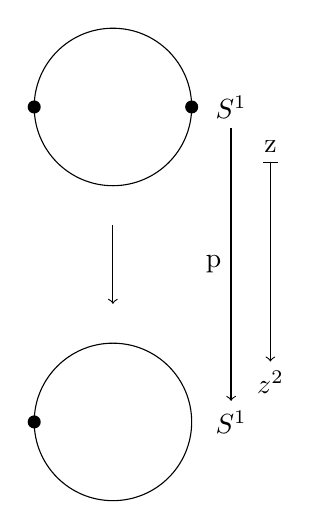
\begin{tikzpicture}
        \draw (0,2) circle (1);
        \node[fill, circle, scale=0.5] at (1,2) {};
        \node[fill, circle, scale=0.5] at (-1,2) {};
        \draw (0,-2) circle (1);
        \node[fill, circle, scale=0.5] at (-1,-2) {};
        \draw[->] (0,0.5) -- (0,-0.5);
        \node (A) at (1.5,2) {$S^1$};
        \node (A1) at (2,1.5) {z};
        \node (B) at (1.5, -2) {$S^1$};
        \node (B1) at (2,-1.5) {$z^2$};
        \draw[->] (A.south) -- (B.north) node[anchor=east, midway] {p};
        \draw[|->] (A1.south) -- (B1.north);
    \end{tikzpicture}
    \qquad
    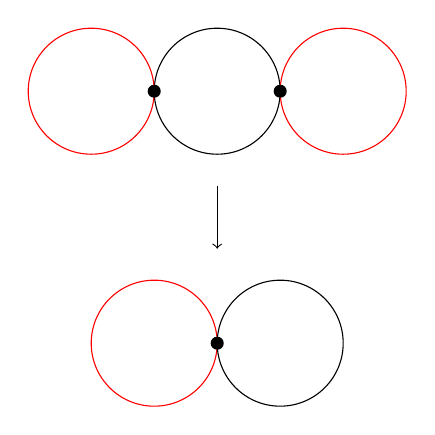
\begin{tikzpicture}[scale=0.8]
        \draw (0,2) circle (1);
        \draw[red] (-2,2) circle (1);
        \draw[red] (2,2) circle (1);
        \node[fill, circle, scale=0.5] at (1,2) {};
        \node[fill, circle, scale=0.5] at (-1,2) {};
        \draw[red] (-1,-2) circle (1);
        \draw (1,-2) circle (1);
        \node[fill, circle, scale=0.5] at (0,-2) {};
        \draw[->] (0,0.5) -- (0,-0.5);
    \end{tikzpicture}
\]
Wir sehen nun, dass die beiden Hebungen der 1-Zelle von $S^1$ nun die beiden 1-Zellen von  $E$ sind. Betrachte nun als zweites Beispiel die rechte Überlagerungen, wobei beide roten Zellen auf die rote abbilden, und die schwarze Zelle mittels $z \mapsto z^2$ abbildet. Dann sehen wir ebenfalls wieder jeweils die beiden Hebungen der beiden Zellen als vier 1-Zellen des Überlagerungsraums.
\end{example}

\begin{example}
    Betrachte die Überlagerung $\R \to  S^1$ durch $z \mapsto e^{iz}$, dann sind zunächst die Hebungen von $S^1$ jeweils die Intervalle  $[n,n+1]$ in  $\R$. Wir erweitern nun zu $S_1 \twedge S^1$ und hängen die entsprechenden Schleifen an den Überlagerungsraum an. Dann ergibt sich folgendes Bild:
    \missingfigure{Überlagerung von $S^1 \twedge S^1$}
\end{example}

\begin{example}[Universelle Überlagerung von $S^1 \twedge S^1$]
    Wir betrachten nun noch die universelle Überlagerung von $S^1 \twedge S^1$, die durch den folgenden Cayley-Graphen von $F_2$ gegeben ist. Man beachte, dass die 'Rekursion' im Bild zwar unendlich fortgesetzt wird, es sich allerdings dennoch nicht um die Teilraumtopologie handelt, die Punkte 'konvergieren' nicht. Wir bilden nun die horizontalen Segmente, die dem Erzeuger $a$ entsprechen, auf den roten Kreis ab, die vertikalen auf den blauen.

\begin{tikzpicture}
    \node (label) at (0,0) {
    \includegraphics[scale=0.25]{figures/600px-Cayley_graph_of_F2.svg.png}
};
    \draw[red] (5,0) circle (1);
    \draw[blue] (7,0) circle (1);
    \node[scale=0.5, fill, circle] at (6,0) {};
    \draw[->] (label.east) -- (3.5, 0);
    \node at (label.south) {\tiny Bild von \cite{img:cayley-graph-f2}};
\end{tikzpicture}
\end{example}

\begin{corollary}\label{cor:untergruppe-von-freier-gruppe-ist-frei}
    Jede Untergruppe einer freien Gruppe ist frei.
\end{corollary}
\begin{proof*}
    Wir können die freie Gruppe durch einen Graphen mit entsprechend vielen Schleifen darstellen. Untergruppen entsprechen nun aber Überlagerungen. Solch eine Überlagerung ist aber  wieder ein Graph und hat damit eine freie Fundamentalgruppe. Also ist die Untergruppe frei!
\end{proof*}

\begin{theorem}[2-dimensionale Komplexe]\label{thm:fundamentalgruppe-von-2-dimensionalem-komplex}
    Sei $X$ ein wegzusammenhängender Raum. Gegebn eine Familie von Abbildungen
     \[
    \left \{\varphi_α \colon  \partial B^2 = S^1 \to X\right\} _{α\in I}
    \] 
    setze
    \[
    Y \coloneqq  X \bigcup_{\left \{\varphi_α\right\} } \coprod_{α\in I} c_α^2
    \] 
    Wähle nun $x_0\in X$, $s_0\in \partial B^2$ und für alle $α$ einen Weg
        \begin{equation*}
        w_α: \left| \begin{array}{c c l} 
            [0,1] & \longrightarrow & X \\
        0 & \longmapsto &  x_0 \\
        1 & \longmapsto \varphi_α(s_0)
        \end{array} \right.
    \end{equation*}
    Dann ist $w_α \circ  \varphi_α(S^1) \circ  w_α^{-1}$ eine Schleife an $x_0$. Sei nun $N \trianglelefteq \pi_1(X)$ der Normalteiler erzeugt von
    \[
        \left \{w_α \varphi_α(S^1)w_α^{-1} \mid  α\in I\right\} 
    \]
    Die inklusionsinduzierte Abbildung
    \[
        \pi_1(X) \to  \pi_1(Y)
    \] 
    ist nun surjektiv mit Kern $N$, d.h.
     \[
         \pi_1(Y) \cong \faktor{\pi_1(X)}{N}
    \] 
\end{theorem}

\begin{example}
    Wähle $X$ als den Einpunktraum und nur eine triviale Schleife. Dann erhalten wir $Y = S^2$, weil wir  $B^2$ entlang des Randes zu einem Punkt verkleben. Der Satz sagt uns nun also:
    \[
        \pi_1(S^2) \cong \faktor{\left< 1 \right> }{\left< 1 \right> } = \left< 1 \right> 
    \]
\end{example}

\begin{example}
    Wir bauen nun den Torus auf, indem wir eine Scheibe entfernen und mittels des Satzes wieder ankleben, siehe hierzu \autoref{fig:torus-mit-ausgeschnittener-scheibe}. Man überlegt sich nun, dass die Relation, entlang derer wir ankleben, $aba^{-1}b^{-1}$ ist, dann ergibt sich als Quotient
    \[
        \pi_1(T^2) \cong \faktor{\pi_1(X)}{\left< aba^{-1}b^{-1} \right> } \cong \Z^2
    \] 

    Wir wissen auch, dass wir den Torus als den Quotienten des Einheitsquadrates schreiben können, das damit eine CW-Struktur aus zwei 1-Zellen und einer 2-Zelle besitzt. Erneut stellen wir fest, dass wir die 2-Zelle entlang $aba^{-1}b^{-1}$ an das 1-Skelett geklebt haben, und wir erhalten wieder $\Z^2$ als Fundamentalgruppe des Torus.
\end{example}

\begin{figure}[ht]
    \centering
    \incfig{torus-mit-ausgeschnittener-scheibe}
    \caption{Torus als $S^1 \twedge S^1$ und angeklebter  $B^2$}
    \label{fig:torus-mit-ausgeschnittener-scheibe}
\end{figure}

\begin{example}
    Wir wissen, dass $\R\mathbb{P}^2$ als CW-Struktur aus einer Schleife hervorgeht, wenn wir die $2$-Zelle entlang  $x \mapsto x^2$ ankleben. Also ergibt sich
    \[
        \pi_1(\R\mathbb{P}^2,x) = \left< a | a^2 \right>  = \faktor{\Z}{2\Z}
    \] 
\end{example}

\begin{corollary}
    Sei $G$ eine Gruppe. Dann existiert ein CW-Komplex mit  $\pi_1(X) \cong G$.
\end{corollary}

\begin{proof}
    Sei $G = \left< E | R \right> $ eine Darstellung der Gruppe. Setze nun $X^0 = \left \{x_0\right\} $ als das 0-Gerüst. Für jeden Erzeuger $e\in E$ kleben wir nun eine 1-Zelle an das 0-Gerüst an, wir erhalten also bereits
    \[
        \pi_1(X^1) \cong \coprod _{i \in I^1 = E} \Z \cong \left< E |  \right> 
    \] 
    Für jede Relation $r\in R$ der Form
    \[
    r = r_1r_2\ldots r_k
    \] 
    mit $r_i \in E$ klebe eine 2-Zelle $c_r$ an  $X^1$ bezüglich der Abbildung
        \begin{equation*}
        \varphi_r: \left| \begin{array}{c c l} 
        \partial B^2 & \longrightarrow & X^1 \\
         & \longmapsto &  r_1r_2\ldots r_k
        \end{array} \right.
    \end{equation*}
    Nach \autoref{thm:fundamentalgruppe-von-2-dimensionalem-komplex} sind wir nun fertig.
\end{proof}

\begin{theorem}[Höhere Zellen zählen nicht]
    Sei $X$ wegzusammenhängend,  $\varphi\colon  \partial B^k \to  X$ stetig mit $k\geq 3$. Setze
    \[
    Y \coloneqq  X \bigcup_{\varphi} B^k
    \] 
    Dann ist die Inklusionsabbildung $\pi_1(X) \to  \pi_1(Y)$ ein Isomorphismus.
\end{theorem}

\begin{corollary}
    Sei $X$ ein wegzusammenhängender CW-Komplex und  $x\in X^0$ ein Basispunkt. Dann ist
    \[
        \pi_1(X, x) = \pi_1(X^2,x)
    \] 
    wobei wir mit $X^2$ das 2-Gerüst von $X$ bezeichnen.
\end{corollary}

\begin{example}
    Wenn wir nun $\R\mathbb{P}^n$ betrachten wollen, so wissen wir, dass es sich um die gleiche 2-Struktur handelt wie die von $\R\mathbb{P}^2$, also wissen wir
    \[
        \pi_1(\R\mathbb{P}^n) \cong \pi_1(\R\mathbb{P}^2) \cong  \Z / 2 \Z
    \] 
\end{example}

\begin{theorem}[Borsuk-Ulam]
    Für jede stetige Abbildung $f\colon  S^2 \to  \R^2$ existiert ein $x\in S^2$ mit $f(x) = f(-x)$.
\end{theorem}

\begin{example}
    Betrachte z.B. die Funktion, die einem Punkt auf der Erdoberfläche seine Temperatur und seinen Luftdruck zuordnet. Dann sagt uns Borsuk-Ulam, dass es zwei Antipoden auf der Erde gibt, die den gleichen Luftdruck und die gleiche Temperatur besitzen.
\end{example}

\begin{proof}
    Angenommen, $f(x) \neq  f(-x)$ für alle $x\in S^2$. Dann ist
        \begin{equation*}
        g: \left| \begin{array}{c c l} 
        S^2 & \longrightarrow & S^1 \\
        x & \longmapsto &  \frac{f(x) - f(-x)}{\norm{f(x) - f(-x)}}
        \end{array} \right.
    \end{equation*}
    wohldefiniert. Wir erhalten nun 
    \[
        g(-x) = \frac{f(-x) - f(x)}{\norm{f(-x)-f(x)}} = - \frac{f(x) - f(-x)}{\norm{f(x)-f(-x)} } = -g(x)
    \] 
    also faktorisiert $g$ und wir erhalten ein  $\overline{g}$, sodass
\[
    \begin{tikzcd}
        S^2 \ar{r}{g} \ar{d}& S^1 \ar[two heads]{d}{p} \\
        \R\mathbb{P}^2 \ar{r}{\overline{g}} & \R\mathbb{P}^1
    \end{tikzcd}
\]
Sei nun $w$ ein Weg von  $x_0\in S^2$ zu $-x_0$. Dann ist $[p(w)] \in \pi_1(\R\mathbb{P}^2, p(x_0)) \cong \Z /2$ ein Erzeuger; die Klasse ist nicht trivial, weil ihre Hebung $w$ keine Schleife ist. Es ist  $g(w)$ ein Weg von  $g(x_0)$ nach $g(-x_0) = -g(x_0)$. Also ist in $\pi_1(\R\mathbb{P}^1, p(g(x_0))$ wieder 

\[
    0 \neq  [p(g(w))] = [\overline{g}(p(w))] = \overline{g}_*[p(w)] = 0
\]
Denn jede Abbildung $\Z / 2 \cong \pi_1(\R \mathbb{P}^2) \to  \pi_1(\R\mathbb{P}^1) \cong \Z$ ist trivial. \contra.
\end{proof}

\begin{corollary}
    $S^2$ ist kein Teilraum von $\R^2$.
\end{corollary}

\begin{remark}
    Das ganze gilt auch für Abbildungen $S^n \to  \R^n$ für jedes $n\geq 1$.

    Für $n=1$ konstruieren wir wie oben  $g\colon  S^1 \to  S^0$, und dann $g(x) = -g(x) \neq  g(x)$, aber $S^1$ ist zusammenhängend und  $S^0$ ist diskret. Also ist jede stetige Abbildung  $S^1 \to  S^0$ konstant.

    Den Fall $n\geq 2$ werden wir in der Topologie I (oder vielleicht auch Topologie II) sehen.
\end{remark}

\section{Ausblick}
Wir haben bereits den Funktior $\pi_1$ kennegelernt, der uns
\[
    \pi_1(S^n) \cong \begin{cases}
        \Z & n = 1 \\
        0 & n \neq 1
    \end{cases}
\] 
liefert. Außerdem wissen wir bereits, dass die $S^n$ beispielsweise als Bausteine von CW-Komplexen von fundamentaler Bedeutung sind.

 \begin{goal}
     Wir wollen für jedes $k\in \N$ einen Funktor $F_k$ mit 
     \[
         F_k(S^n) \cong \begin{cases}
             \Z & k = n \\
             0 & \text{sonst}
         \end{cases}
     \]
     konstruieren.
\end{goal}

\begin{warning}
    Man käme in Versuchung, $F_k = \pi_k$ zu setzen, das funktioniert aber nicht, denn es ist z.B. $\pi_3(S^2) \neq  0$.
\end{warning}

Es sei angemerkt, dass $\pi_k$ trotzdem interessant, allerdings \emphasize{sehr} schwer zu berechnen.

Stattdessen betrachten wir \vocab{Homologie}, notiert $H_{\bullet}$, diese ist
\begin{itemize}
    \item schwieriger zu definieren
    \item relativ leicht zu berechnen, insbesondere für CW-Komplexe
    \item immer abelsch
\end{itemize}
Dual dazu gibt es die sogenannte \vocab{Kohomologie}, notiert $H^{\bullet}$.
\begin{itemize}
    \item Diese hat noch mehr Struktur, z.B. eine Ringstruktur.
    \item Damit können wir z.B. den Fall $n\geq 2$ von Borsuk-Ulam zeigen.
\end{itemize}

In Topologie I werden wir nun $H_{\bullet}$ und $H^{\bullet}$ einführen und wichtige Sätze über sie beweisen.

In der Topologie II  werden wir die Homologie von Mannigfaltigkeiten, insbesondere die Poincare-Dualität, untersuchen. Ebenfalls werden wir den Zusammenhang zwischen $\pi_n$und $H_n$ untersuchen.
